\textbf{Abstract} The connectivity is of paramount importance to a network, whose basic function is to route packets between end points.  
Junda Liu et al. proposed Data-Driven Connectivity (DDC) to ensure routing connectivity via data plane mechanisms, which allows networks to provide a much higher degree of availability, while still providing flexible routing control~\cite{liu2013ensuring}.
Nowadays, against the backdrop of the development of P4, Programming Protocol-independent Packet Processors (a domain-specific language)~\cite{P4}, one can enable the programmabilitiy of network devices to perform simple but extremely fast packet processing directly in the data plane.
This article is a replication work of~\cite{liu2013ensuring} within P4 ecosystem. 
Specifically, we implement DDC to the behavioral model version 2 (BMv2), a P4-based and vastly used software switch. We evaluate our implementation against several benchmarks from the original paper, and we find that our results essentially align with the original work.  

\section{Introduction}

In the domain of computer networks, we typically disassociate the forwarding process of network packets in the so-called \textit{data plane}, from the routing process in the \textit{control plane}. 
While the control plane determines how packets should be forwarded, the data plane actually forwards the packets. 
By this division of concerns, it is the control plane that takes the burden of ensuring connectivity.  
In terms of timescales, nevertheless, packet forwarding operates above thousands of times faster than the convergence of control plane protocols when faced with failures~\cite{liu2013ensuring}. 
Long outages, during which the control plane computes new paths and installs them into routers, will bring inevitable damages. 
Even though there exist approaches that pre-compute some backup paths (ECMP, MPLS's Fast Reroute, etc.), which might satisfy most customer requirements, rigorous network resilience still lacks sufficient guarantees.

In order to tackle these outlined deficits, the paper~\cite{liu2013ensuring} proposes the idea of \textit{Data-Driven Connectivity} (\textbf{DDC}) which maintains ideal forwarding connectivity at the data plane time-scales. 
DDC, employing only simple bit manipulation operations in the data packet headers, leaves network functions that require global views (optimizing routes, etc.) to the control plane and moves connectivity maintenance, which has simple yet radical semantics, to the fast data plane. 
Traditionally, the data plane has been designed with fixed functions applying a limited set of protocols, which has largely constrained the flexibility of implementations. 
The recent availability of P4, which stands for \textit{Programming Protocol-independent Packet Processors}~\cite{P4}, has enabled the programmability of data plane, which drastically upgrade the efficiency of customizing, testing and adopting new network applications. 

Therefore, we proceed to re-implement DDC and evaluate the entire system in P4, attempt to replicate the test results and clarify the unclear yet crucial details in the paper. 
The background and scope of our replication work are summarized in Section 2. 
The complete DDC algorithm is introduced in Section 3.
Section 4 illustrates, in details, our implementation of DDC and its control plane. 
Finally, the evaluation result via several benchmarks is presented and is compared with the original paper.


\section{Scope of Reproducibility}
\textbf{Replication Background} Authors of the paper~\cite{liu2013ensuring} have provided their complete NS-3 codes~\cite{ddc-ns3}. But since P4 is highly differentiated from other languages, there isn't much to refer from this code. After the contact with the authors, we found someone has implemented DDC in  $ \rm {P4}_{14}$~\cite{ddc-p4} for the Intel Tofino switch~\cite{Tofino}. However, as many proprietary libraries (e.g. stateful ALUs) used in this code are commercial and not open-source, the obscurity in this implementation leads to the lack of the universality. And  nowadays, $\rm P4_{16}$ is supported for most P4-programmable target devices.

Thus, we decided to re-implement the entire DDC algorithm in $\rm P4_{16}$ on a widely applied software target, behavioral model version 2 (\textbf{BMv2}), which is developed by the P4 community. In the framework proposed by the original paper, while DDC plays the foremost role which guarantees the connectivity, a set of optimizations are implemented in the control plane to steer the data plane algorithms towards selecting better paths. We have re-implemented a part of the control plane optimizations stated in the paper, and we also obtained the results with similar performance indications. Additionally, the whole implementation has been evaluated via two benchmarks, i.e.\ path stretch and packet latency, on different topologies.

\section{DDC Algorithm}
DDC algorithm serves at its core to ensure ideal connectivity with data plane mechanisms, which aims to guide all the paths on a directed acyclic graph (\textbf{DAG}) to the specified destination by sets of \textit{link reversal} operations. From a high level point of view, the DDC algorithm:
\begin{itemize}
    \item[-] takes an arbitrary DAG per destination in the network as inputs
    \item[-] returns a \textit{destination-oriented} DAG per destination in the network as outputs
    \item[-] and guarantees that all packets get forwarded and eventually reach their destinations based on the corresponding DAG, in spite of link failures (as long as the network remains connected).  
\end{itemize}
The algorithmic foundations of DDC lie in classic Gafni-Bertsekas (\textbf{GB}) link reversal~\cite{GB} routing. Generally, link reversal encompasses two types of algorithms, one is full reversal, another is partial reversal. 
\begin{itemize}
    \item \textbf{Full reversal}. At each iteration, each node other than the destination that has no outgoing link reverses the directions of all its incoming links. 
    \item \textbf{Partial reversal}. Every node $i$ other than the destination keeps a list of its neighboring nodes $j$ that have reversed the direction of the corresponding links $(i, j)$. At each iteration, each node $i$ that has no outgoing link reverses the directions of the links $(i, j)$ for all $j$ which do not appear on its list, and empties the list. If no such $j$ exists (i.e., the list is full), node $i$ reverses the directions of all incoming links and empties the list. 
\end{itemize} 
DDC essentially utilizes the partial reversal for reducing the quantity of operations. Figure 1 provides an example of successive iterations of the partial link reversal algorithm. Initially, the desitination-oriented DAG is stable until a link fails. Then the nodes, labeled with $R$, that have no outward links will reverse all its links, except the links have already been reversed at the last step. Eventually, after several iterations, the DAG is converged to be destination-oriented again.

\begin{figure}[H]
      \centering 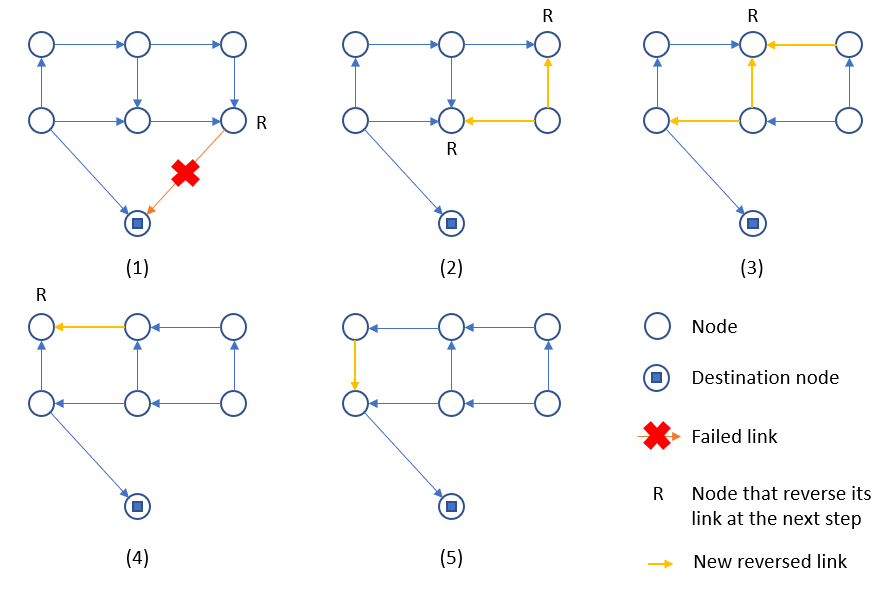
\includegraphics[scale=0.65]{pictures/partial reversal.png}
      \caption{\it{Link Reversal Algorithm (Partial reversal)}}
\end{figure}

However, GB is not plausible for the data plane. For instance, it involves generating special control packets, potentially sent to a large number of neighbors, and do not handle packets losses. DDC has made some crucial enhancements to handle packets losses and delays and also make it work on the packet-forwarding timescales. DDC algorithm is stated in details as follows.\\

\textbf{State at each node:}
\begin{itemize}
    \item to\_reverse: List recording the reversed links at last iteration, initialized to the incoming links of a given graph $G$. 
    \item direction[L]: In or Out, represents this node's view of the direction of link $L$.
    \item local\_seq[L]: One-bit unsigned integer, initialized to 0, associated with this node's view of link $L$'s direction.
    \item remote\_seq[L]: One-bit unsigned integer, initialized to 0, associated with the view of the neighbor at the other end of link $L$.
\end{itemize}

\textbf{State in packets:}
\begin{itemize}
    \item packet\_seq: One-bit unsigned integer; when packet is sent, set as sender node's local\_seq; when packet is arrived, set to be compared with receiver node's remote\_seq.  
\end{itemize}

The pseudo code of DDC shows as below. 


\begin{algorithm}[]
    \newcommand{\INDSTATE}[1][1]{\STATE\hspace{#1\algorithmicindent}}
    \caption{DDC}
    \begin{algorithmic}[1]
    \label{algo:DDC}
    
    {\small
    \linenumbers
        \INDSTATE packet p generated locally:
            \INDSTATE[2] update\_FIB\_on\_departure() \
            \INDSTATE[2] send\_on\_outlink(any outlink, p) \\[0.1in]
        \INDSTATE packet p received on link L:
            \INDSTATE[2] update\_FIB\_on\_arrival(p, L) \
            \INDSTATE[2] update\_FIB\_on\_departure() \
            \INDSTATE[2] if (direction[L] = Out) \
            \INDSTATE[4] if (p.seq == remote\_seq[L])
            \INDSTATE[6] send\_on\_outlink(L, p)
            \INDSTATE[4] \linelabel{algo:any out link}send\_on\_outlink(any outlink, p) 
        \\[0.1in]
        \INDSTATE send\_on\_outlink(link L, packet p)
        \INDSTATE[2] p.seq = local\_seq[L]
        \INDSTATE[2] send p on L
        \\[0.1in]
        \INDSTATE reverse\_in\_to\_out(L)
        \INDSTATE[2] direction[L] = Out
        \INDSTATE[2] local\_seq[L]++
        \\[0.1in]
        \INDSTATE reverse\_out\_to\_in(L)
        \INDSTATE[2] direction[L] = In
        \INDSTATE[2] remote\_seq[L]++
        \\[0.1in]
        \INDSTATE update\_FIB\_on\_arrival(packet p, link L)
        \INDSTATE[2] if (direction[L] = In)
        \INDSTATE[4] assert(p.seq == remote\_seq[L])
        \INDSTATE[2] else if (p.seq != remote\_seq[L])
        \INDSTATE[4] reverse\_out\_to\_in(L)
        \\[0.1in]
        \INDSTATE update\_FIB\_on\_departure()
        \INDSTATE[2] if there are no Out links
        \INDSTATE[4] if to\_reverse is empty // partial reversal impossible
        \INDSTATE[6] to\_reverse = all links
        \INDSTATE[2] for all links L in to\_reverse
        \INDSTATE[4] reverse\_in\_to\_out(L) // Reset reversible links
        \INDSTATE[4] to\_reverse = \{L: direction[L] = In\}}
    \end{algorithmic}
\end{algorithm}

\section{DDC Implementation}

\subsection{DDC in P4}
\label{sec:DDC}
\subsubsection{Packet Header}
We assume that the packets coming from each host are in standard header format, i.e.~ETHERNET/IP/TCP(UDP)/. To make use of DDC algorithm as a routing approach, DDC layer is inserted into the packet header between layer 2 and layer 3, i.e.~ETHERNET/DDC/IP/. The inserting operation is conducted by p4 switches which are directly neighbored to the hosts. For a packet whose last hop is the source host arrives at the neighbor switch, DDC will be set valid to guide the network behaviors. Hence, this kind of switch is regarded as \textit{border switch}, which also removes DDC header if the next hop of a packet is the destination host. In addition, the link connecting a host and a switch should be excluded from consideration when choosing out links to forward based on DDC due to that this sort of links are absent from the area that DDC is validated.

\begin{figure}[H]
      \centering 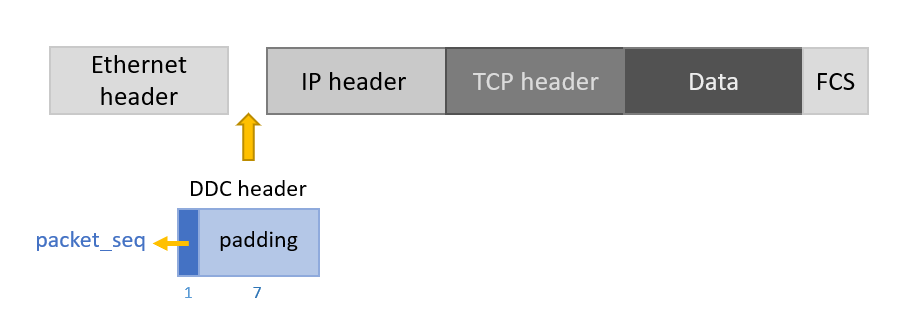
\includegraphics[scale=0.55]{pictures/packet header.png}
      \caption{\it{Packet header}}
\end{figure}

DDC header is mainly a 1-bit packet\_seq, and for the reason that BMv2 target only supports headers with fields totaling a multiple of 8 bits (!!Add a cite to spec), we also add a 7-bit padding part.    

\subsubsection{Data Structures}
We used sequential bits to represent the \ls, \rs, \ld, and \tr of each node. Within the bits instance, each bit represents the corresponding info  of each link on this node. The length of bits relies on the maximum link quantity of the node (generally 32-bit). For example, 
\begin{itemize}
\item if \ls is X...X01, it means the \ls of the link on port 1 is 1 while that on port 2 is 0.
\item if \ld is X...X01, it means the direction of the link on port 1 is in while that on port 2 is out.
\item if \tr is X...X01, it means the link on port 1 should be regarded as a potential option to be reversed, while that on port 2 should not.
\end{itemize}
Most constructs in P4 are stateless, which means given some inputs they produce a result that solely depends on these inputs. Thus, as a packet processing language, once it completes handling the information within each incoming packet and transfers it out, normally this information is not stored. However, the states at each node, such as \ls and \rs, should be retained across sending and receiving of packets. To this end, here we use the register, a stateful extern object, in v1model architecture(add a citation!!!), that has states which can be read and written by both control plane and data plane. Registers are assigned in arrays and useful for storing small amounts of arbitrary data. As the DAG is per-destination based, it is necessary to store these states respectively for different destinations. So we initialize a register for every state, each of which possesses elements of maximum destination quantity in the array format. \\

In the light of that P4 supports neither the \textit{for} loop nor other advanced data structures, storing the state information in the sequential bits and indexing them by disparate destinations is the most efficient and plausible way to re-implement DDC algorithm in P4. According to this, we need to frequently take bit operations, including shift\_left, shift\_right, AND, OR.  For instance, to judge whether a link\_direction is certainly in or out, simply shift left 1 to the corresponding bit position and use OR logic with original bits to compare; to judge whether packet\_seq (1-bit) is equal to the remote\_seq on the arriving port, shift\_left the packet\_seq, use AND logic to get the needed bit of remote\_seq while masking others and then make a comparison.

\subsubsection{Process Flow}
Typically, a P4 program contains a parsing state that extracts packet headers, an ingress and egress control block that modify packets, and a deparsing state that assembles modified packets. Within the control blocks, the bits extracted at the parser state can be manipulated and transformed. In our implementation, we create another two control blocks to update \textit{forwarding information base} (FIB) upon both departure and arrival, which will be invoked at the ingress control. In the control block, we can define and invoke the action, similar to a function in other languages, and the table, a special construct in P4 that is regarded as a match-action unit which associates user-defined keys with actions. Therefore, we implement the function blocks in the DDC algorithm as either tables or actions. \\
In the process flow of our implementation illustrated in \Cref{fig:p4Process} (the drawing is inspired from~\cite{CS344}), if the packet originated from the hosts reaches the border switch, DDC header will be added within the ingress control. Then with the premise of valid DDC header, the extracted bits and metadata will go through two updating control blocks to renew the FIB and reverse the links (if necessary), out links to forward will be determined on the basis of states information. Once this packet eventually reaches the border switch connected to the destination host, at the egress control, after setting DDC header invalid, we recirculate the packet to the ingress control to get the forwarding decision made by the longest prefix match of ipv4 forwarding rather by DDC.

\begin{figure}[H]
      \centering 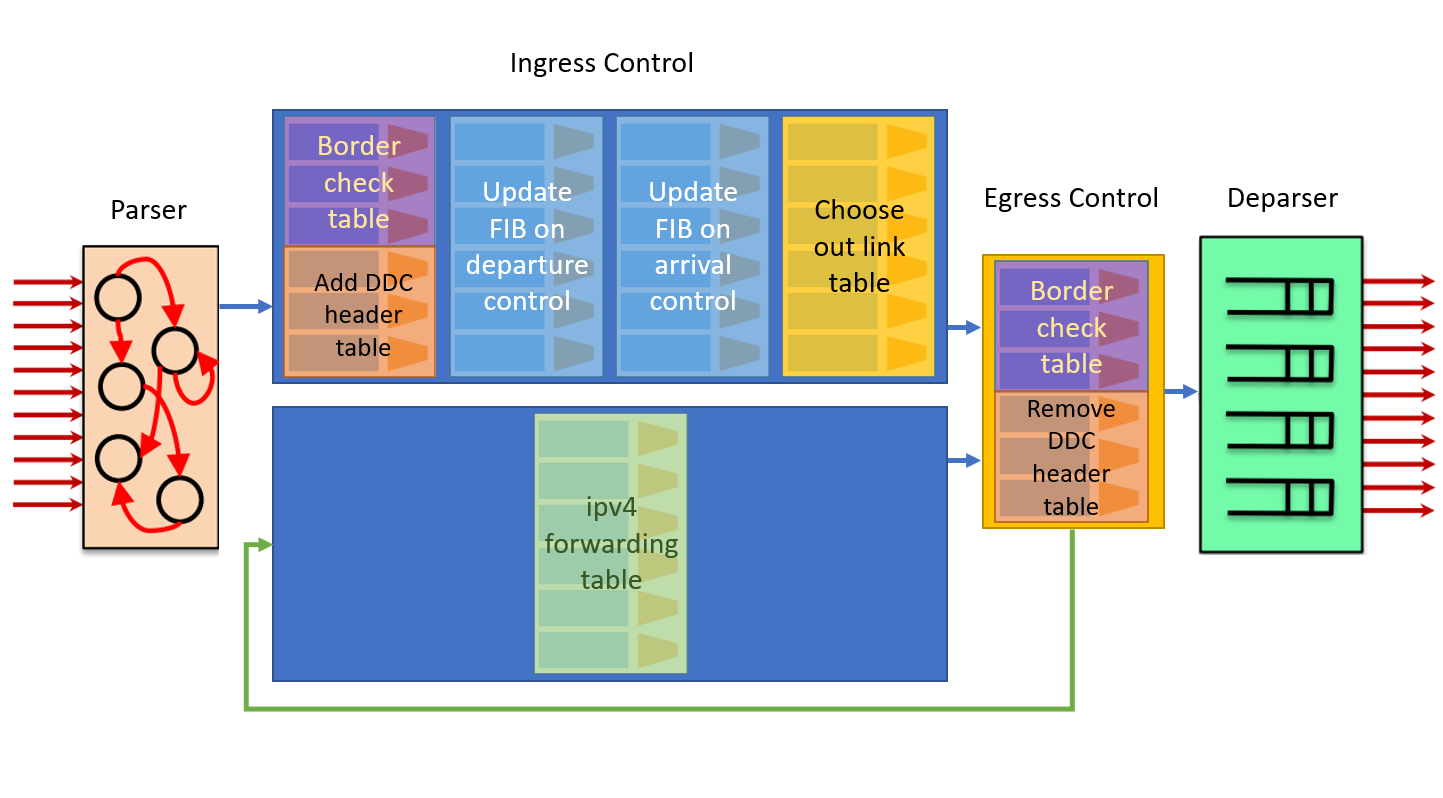
\includegraphics[scale=0.44]{pictures/process flow.png}
      \caption{\it{P4 Process Flow}}
      \label{fig:p4Process}
\end{figure}

\subsection{Control Plane Implementation}
\label{sec:control}
DDC guarantees connectivity in the data plane, but it also relies on the control plane to guide the data plane to use desirable paths. A P4 program represents only a part of a complete working system. The control plane software is written in one or more general purpose programming languages like C, C++, Python, etc., and is responsible for adding and removing entries to P4 tables. 

We make a large use of \textit{P4-utils}~\cite{p4-utils} (in Python), which creates virtual networks using mininet~\cite{mininet} (a network virtualization engine that is convenient to deploy Software-Defined Networking systems) and extended nodes that run p4-enabled switches. Mininet takes bash processes to create hosts in an isolated network namespace and uses virtual ethernet pairs, living in the Linux kernel, to connect the emulated hosts with our BMv2 switches. \textit{P4-utils} also provides multiple gainful APIs to write controllers (e.g., analyzing topology, adding table entries and writing/reading values into/from registers), by which we install the table entries and initialize register values. The following subsections detail how the \ld registers are initialized, and how edge priorities are implemented.

\subsubsection{Initialization of the destination-oriented DAG}
Packets serve as reversal notifications in the data plane algorithm. Although DDC is absolutely feasible on an initially arbitrary DAG, it is practically efficient to initialize a (converged) destination-oriented DAG for the purpose of decreasing the time of packets probing. The original paper proposes the all-edges-outward (\textbf{AEO}) operation, which modifies all of a single node’s edges to point outward. Let assume that each node is assigned a \textit{distance} from the destination. These could be produced, for instance, by a standard shortest path protocol or by a central coordinator.  Let $v_1$,...,$v_n$ be the (non-destination) nodes sorted in order of distance from the destination, i.e., a topological sort of the target DAG. Suppose we iterate through each node $i$ from 1 to $n$, performing an AEO operation on each $v_i$, as showed in \Cref{fig:AEO}. The resulting destination-oriented DAG contains only shortest paths to the destination, because for any undirected edge ($u$,$v$) such that $u$ is closer to the destination, $v$ will direct the edge $v \rightarrow u$ after $u$ directed it $u \rightarrow v$.

\begin{figure}[H]
      \centering 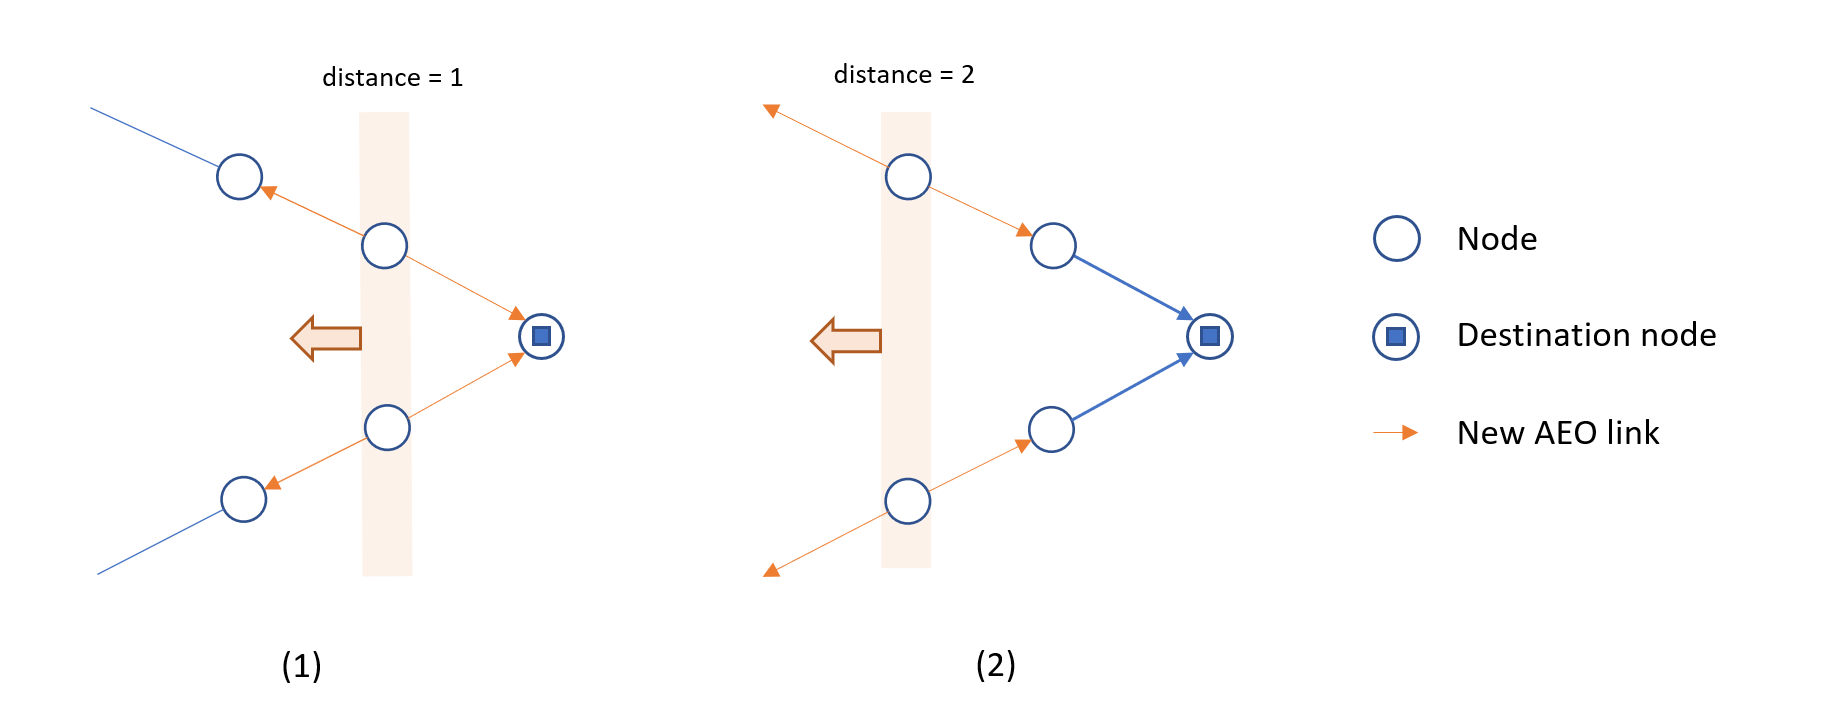
\includegraphics[scale=0.36]{pictures/AEO.png}
      \caption{\it{AEO operation}}
      \label{fig:AEO}
\end{figure}

In the controller code, we implement Dijkstra's algorithm~\cite{dijkstra1959note} upon the network topology to get the distances of each source-destination pair, from which the order of nodes is obtained for each destination-oriented DAG. AEO operations, then, are implemented by writing (modifying) the respective corresponding values into \ld registers of two nodes on the link, which ensures that these two nodes have stable consensus on the direction of interconnected link.  

\subsubsection{Edge priority}

DDC algorithm allows for the use of an arbitrary output link, i.e., packets can be sent out any output link ( \hyperref[algo:DDC]{line 3, 10} in the pseudo code). To accomplish greater efficiency, such as faster convergence and traffic engineering, the choice of output links can be optimized by a control-plane specified priority, which can be set by some global computation or manual operator preferences. 

The original paper doesn't explain how edge priority is set while it is necessarily implemented in their evaluation tests. In our work, grounded on Dijkstra's algorithm, we can have the paths and distances of any two nodes. Let $dist(p)$ represents the distance from the port $p$ of source to the destination. Obviously, in \Cref{fig:edge prios}, the link on port 1 is at the lowest priority while that on port 2 is at the highest. 

Even though one can install the general table rules with multiple priorities (i.e., by declaring \textit{prios} when adding table entries), doing so is not plausible for per-destination based edge priorities. To this end, we define five registers (also indexed by destinations) for each switch controller, in which the port number with five highest priorities will be written respectively. For instance, if the prioritized port numbers of a switch to the 1st destination are 3,4,1.., then upon this switch, the 1st element in \textit{edge\_priority\_0} is X..X0100, in \textit{edge\_priority\_1} is X..X1000, in \textit{edge\_priority\_2} is X..X0001, etc. When choosing the output link, it could first check if the direction of a prioritized link is out. If so, output port number is decided. 

There are two reasons that we only define five registers. One is that computing all possible paths between all pairs of nodes does not scale, and becomes intractable when applied to real network topologies; thus, we turn to only compute the shortest paths among them. Given the list of the shortest paths, these registers are enough to store the prioritized ports while some of them are empty. 
The second reason is that, since loops are not supported in P4, there is no choice but to check these edge priority registers repetitively one by one. In practice, we found that having five link options is already sufficient for classical link failure scenarios. 

\begin{figure}[H]
      \centering 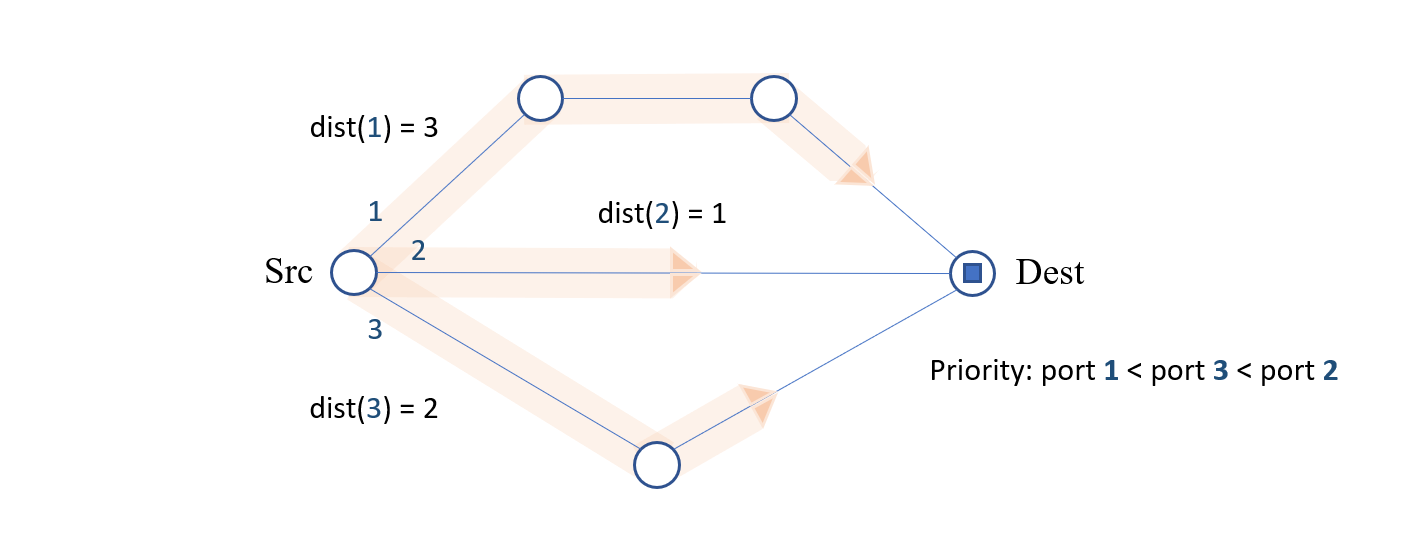
\includegraphics[scale=0.40]{pictures/edge prios.png}
      \caption{\it{Example of edge priority}}
      \label{fig:edge prios}
\end{figure}


\section{Evaluation}
We replicate the DDC evaluation tests via two benchmarks, path stretch and packet latency. To stay consistent with the original paper, we only evaluate shortest-path DAGs and set the edge priorities described in \cref{sec:control} to minimize path length. 
In overall, we obtain similar results as presented in the original paper. 

\subsection{Link Failure Implementation}
Testing under link failure scenarios is an indispensable part for the whole evaluation of DDC performance. To simulate link failures, we get inspired from the \textit{Fast-Reroute}~\cite{12-Fast-Reroute} exercise in the lecture, Advanced Topics in Communication Networks~\cite{adv-net}, taught at ETH Zurich. By building a command line interface (\textbf{CLI}) to introduce failures, executing commands, e.g., fail s1 s2, can automatically update the \lkst registers of switch 1 and switch 2. The \lkst, which namely represents the link states (i.e, up or down) of a node, is taken as another necessary condition while choosing output links, i.e., an output port can be chosen when and only when the \ld is out and the \lkst is not down. The delay between the failure and controller updates is not simulated here, because in practice, the controller can be notified very quickly (i.e., hundreds of milliseconds) using data-plane techniques such as BFD~\cite{rfc5880}. 

\subsection{Path Stretch}
Path stretch is defined as the ratio between the length of the path a packet takes through the network, and the shortest path between the packet’s source and destination in the current network state, which is useful to evaluate the performance of DDC under failure scenarios. 
As the Dijkstra's algorithm can compute the length of the shortest paths, the main task left is to obtain the length of the path packets take. 
To solve this, we insert a 32-bit \hp field into the header to record the quantity of hops that packet traversed through. At each time that the routing decision is made by DDC, the \hp increases by 1. Once it reaches the border switch next to the destination host, the value will be written into a \hn register indexed by source hosts. By the simple switch CLI implemented in \textit{p4-utils}, we can read this value from the \hn register of the border switch. 

We select 200 random source-destination pairs, and fail links on the connecting paths. A series of packets are sent out (one at a time to avoid congestion drops), the path of which changes as DDC routes after failures. To know which paths should be exactly failed, we simulate the routing operations in the controller to compute the actual paths. This is accomplished by choosing the output port based on the values read from \ld and \lkst registers, mapping the port to the interface, transforming it into the connected node, and then repeating procedures above until the packet reaches the destination. 

We essentially evaluate our implementation on AS1239's topology, which contains 361 nodes and 1479 links (topology data is provided in the author's GitHub~\cite{ddc-ns3}), both with and without edge priority. 
250 hosts are deployed here because BMv2 target only supports 256 host instances. 
The bit length of DDC parameters such as \ls, \rs are also prolonged to 40-bit due to that in this topology, the maximum links on a node is 39. 
As showed in \Cref{fig:pathStretch}, we can find that edge priority obviously optimizes the stretch performance, and the holistic trend is to a large extent akin to the result in the original paper: after the $8^{th}$ packet, the path stretch gets close to 1. 
The $99^{th}$ percentile initial stretch is around 6 while that in the original paper is 14. 

Moreover, we also attempt to replicate the results on a data-center topology, FatTree~\cite{FatTree}. 
In the original work, they failed 10 links on the paths between two nodes.
However, the maximum path length in this topology (grounded on the data provided in the author's GitHub) is 4, i.e., two up and two down, therefore, it is unclear how the failed 10 links are chosen.
We try failing 4 links, but the routing mechanism of DDC immediately switches to another equivalently desirable path in 4-hops as well, which maintains path stretch at 1. 
To sum up, it is rather ambiguous what experimental settings the authors used to observe an effect of failure on the path stretch in the FatTree topology.

\begin{figure}[H]
      \centering 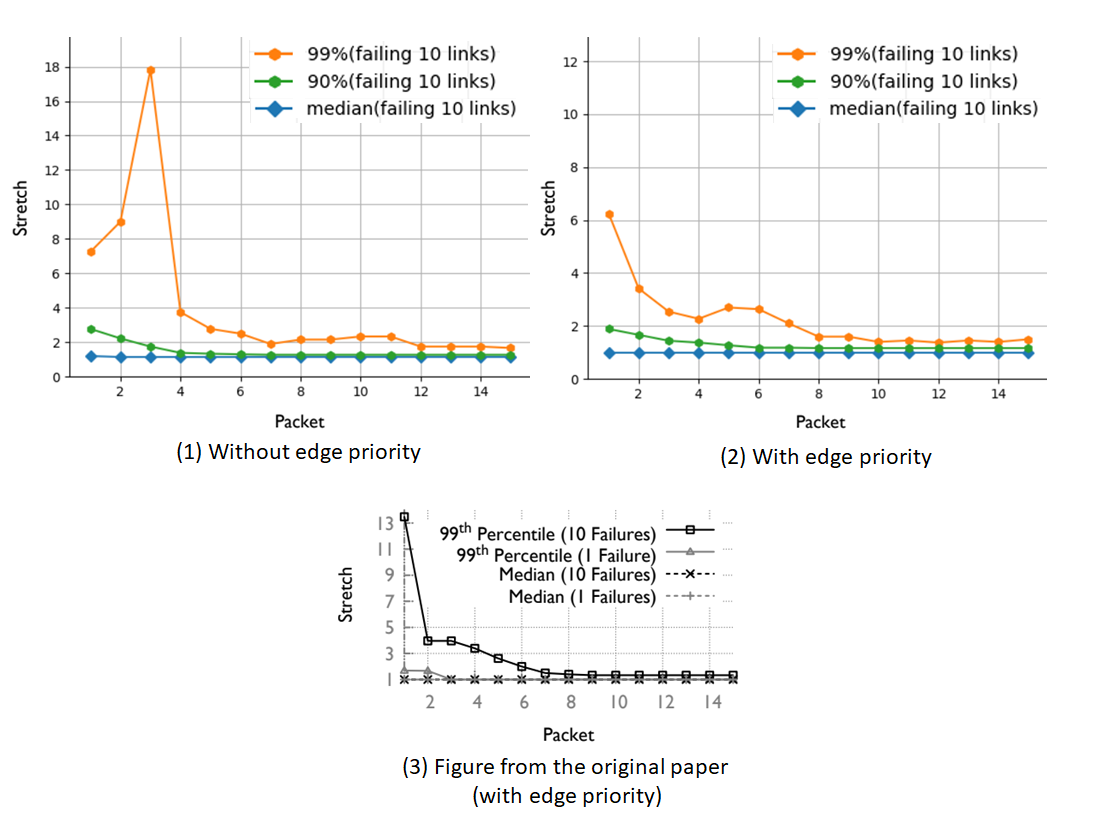
\includegraphics[scale=0.58]{pictures/pathStretch.png}
      \caption{\it{Median and $99^{th}$ percentile stretch for AS1239}}
      \label{fig:pathStretch}
\end{figure}

\subsection{Packet Latency}
The DDC algorithm may also impact packet latency by increasing queuing at certain links as it moves packets away from failures. 
Thus we measure the temporary effect by comparing the time taken to deliver a packet before and after failures. 
To measure this, we use 30 random source nodes sending 1GB of UDP traffic each to 10 randomly chosen destinations using a data rate of 4Mbps  during 25s. 
All links are configured with a capacity of 10Mbps and a propagation delay of 10ms.
These settings are similar to those from the original paper.

For each source-destination pair, we measure latency in the normal situation, with 2 link failures and with 10 link failures respectively. 
Because each Mininet host is essentially a bash shell process attached to one or more network interfaces, we take advantage of the scapy and socket Python libraries to build \textit{send.py} and \textit{receive.py} to be invoked by the host. 
To enter into the same network namespace, writing commands, e.g., \textit{h1 python send.py}, \textit{h2 python receive.py}, to the Mininet CLI will instruct host 1 to send traffic and host 2 to receive traffic. 
By comparing the time of sending and receiving, the packet latency is computed. To execute these two commands at the same time, putting \& at the end of command can dispose it to the background.

We evaluate on AS2914's topology (454 nodes, 1543 links). 
According to the cumulative distribution function (\textbf{CDF}) result illustrated in \Cref{fig:pktLatency}, it is indicated that about 85\% of packets encounter a modest increase in latency while in the original work it reaches 96\%. 
There exists a trivial deviation of time in terms of the clock of distributed hosts, but the general performance in latency is consistent with the original work.


\begin{figure}[H]
      \centering 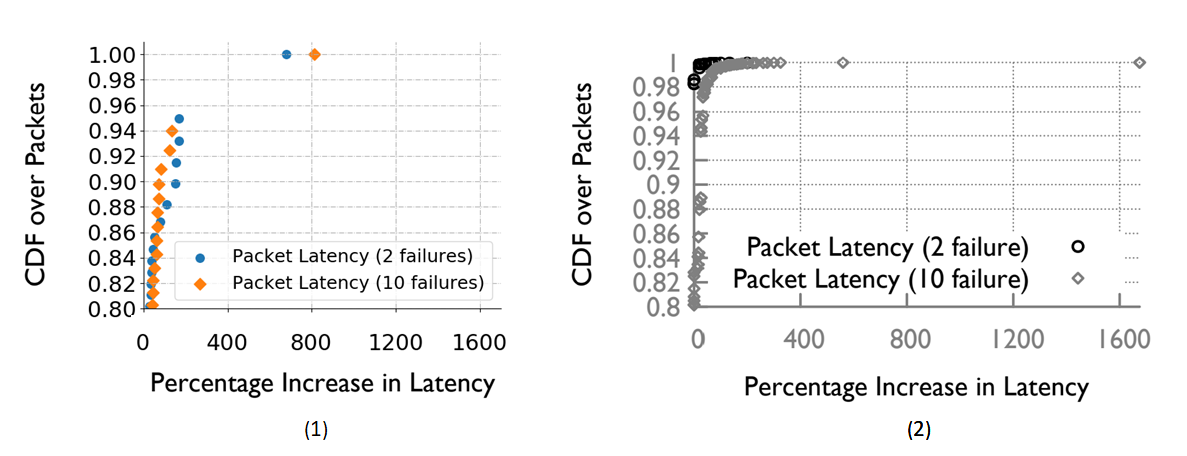
\includegraphics[scale=0.52]{pictures/pktLatency.png}
      \caption{\it{Packet latencies in AS2914 with link failures\\(1)Our result (2)Figure from the original paper}}
      \label{fig:pktLatency}
\end{figure}

\section{Discussion}

\subsection{What was easy}
The overall structure of the original paper is well-organised and straightforward to follow. Due to the brevity and clarity of DDC itself, the re-implementation of the algorithm is not particularly difficult. 
With the collaboration of the authors, we confirmed that there is a typo in the original manuscript (i.e., at \hyperref[algo:DDC]{line 8} of pseudocode, it should be $==$ rather than $!=$).
The $\rm P4_{14}$ code for Tofino also provided some inspiration for our replication at the initial stage.

\subsection{What was difficult}
The whole replication lies in the P4 ecosystem while the original work was done in NS3 (mainly in C++), which requires us to transform the way of thinking and implementation. 
Though the P4 syntax is not very complicated, there exist some limitations on the data structure (e.g., no support for loops and limited state retention), which requires to properly make use of proprietary structures and external libraries (e.g., registers). 
Debugging a P4 program mainly consists in checking the log file (with thousands of lines) of each switch, which is to some extent inconvenient.

The P4 ecosystem doesn't offer mature tools or interfaces to monitor the network behaviours, and as aforementioned, a P4 program only represents a fraction of a complete working system, it takes some efforts to design the evaluation framework for benchmarks and pack up those procedures into automation. 

Furthermore, some crucial part for evaluation were not detailed in the original paper, which led to uncertainty in the concrete experiment setup. 
For instance, how to assign priority to the port in practice? In a FatTree topology, how to fail 10 links on an existing path whereas the maximum path length is 4? In the packet latency experiment, how to set the sending rate of hosts to guarantee that links are used no more than 50\% of the capacity? Ultimately, almost all the experiments presented in the paper are under-specified to a certain extent, which made exact replication difficult.


\section{Conclusion}
In this work, we successfully re-implement the DDC algorithm in an uprising data-plane language, $\rm P4_{16}$, and apply it on the widely used and open-source BMv2 software switch. 
We also design and provide complete approaches for the evaluation via benchmarks, and replicate part of its simulation results within P4 ecosystem, which confirms the benefits of DDC. 

Our re-implementation is open-source (data and codes are provided at this repository \cite{repo}). 
We hope that this replication can help clarify the methods of re-implementing the DDC mechanism, and that it can promote future research in the domain.